\documentclass{beamer}

\mode<presentation> {
  \usetheme{Warsaw}
  \setbeamercovered{transparent}
}

\usepackage[french]{babel}
\usepackage[latin1]{inputenc}

\usepackage{amsmath,amssymb}
\usepackage{graphicx}
\usepackage{fancyvrb}


\title{Le Grand Londres \textbf{Beamer}}

\author{ASRALL 2017 -\LaTeX}

\date{IUT Nancy-Charlemagne} %

\subject{Outils libres}

\pgfdeclareimage[height=0.8cm]{university-logo}{logo}
\logo{
\includegraphics[width=8mm]{./img-slides/un.jpg}}



%\beamerdefaultoverlayspecification{<+->}

\begin{document}

\begin{frame}
  \titlepage
\end{frame}


\begin{frame}
  \frametitle{Plan}
  \tableofcontents[pausesections]
\end{frame}


\section{Introduction}

\subsection{Londres}

\subsection{D�finition de Londres}

\begin{frame}
    \frametitle{Introduction}
%\begin{block}{G�n�ral}
Londres, situ�e dans le sud-est de la Grande-Bretagne, est la capitale et la plus grande ville de l'Angleterre et du Royaume-Uni. Longtemps capitale de l'Empire britannique, elle est d�sormais le si�ge du Commonwealth of Nations
%\end{block}
\begin{center}
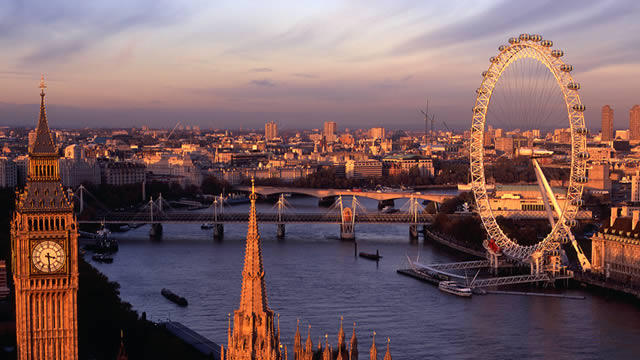
\includegraphics[width=0.6\textwidth]{./img-slides/londres.jpg}
\end{center}
\end{frame}

\begin{frame}
\begin{columns}
 \begin{column}{0.55\textwidth}
\begin{block}{Sites d'int�r�t}
    \begin{enumerate}[<+-| alert@+>]
      \item  Big Ben
      \item  Le soir dans la ville
      \item  St. Pancras
    \end{enumerate}
\end{block}
 \end{column} \ \
 \begin{column}{0.40\textwidth}
      \only<1>{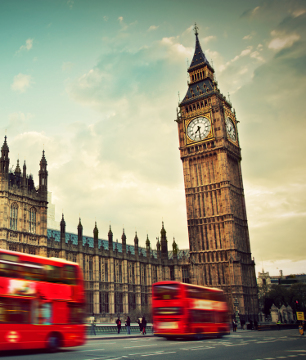
\includegraphics[width=0.8\textwidth]{./img-slides/deux.jpg}}
      \only<2>{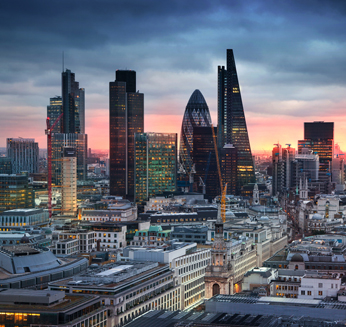
\includegraphics[width=0.9\textwidth]{./img-slides/trois.jpg}}
      \only<3>{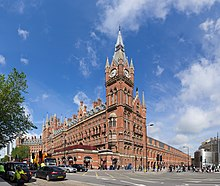
\includegraphics[width=0.9\textwidth]{./img-slides/quatre.jpg}}
 \end{column}
\end{columns}
\end{frame}

\section{G�ographie}

\subsection{Relief et hydrographie}

\begin{frame}
    \frametitle{Relief et hydrographie}
\begin{block}{}
La d�nomination courante Londres peut d�signer plusieurs ensembles g�ographiques ou administratifs diff�rents, pouvant parfois porter � confusion.
\end{block}
\begin{center}
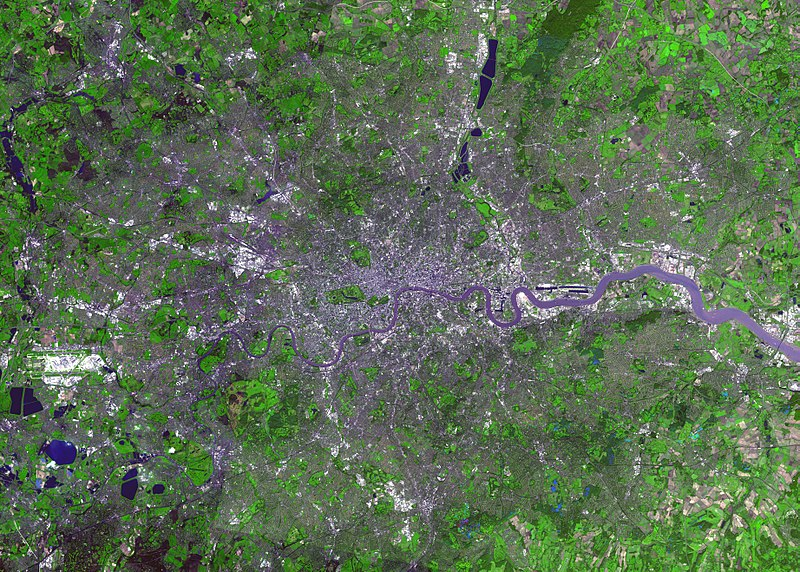
\includegraphics[width=0.5\textwidth]{./img-slides/relief.jpg}
\end{center}

\end{frame}


\subsection{Quartiers}

\begin{frame}
    \frametitle{Quartiers}
\begin{block}{}
On d�crit souvent Londres par quartiers (Bloomsbury, Mayfair, Whitechapel par exemple). Ces noms n'ont pas d'utilisation officielle mais d�signent souvent des paroisses et sont rest�s en usage par tradition.
\end{block}
\begin{center}
\begin{figure}
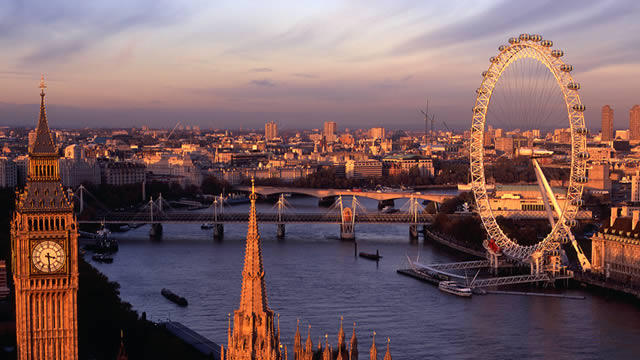
\includegraphics[width=0.3\textwidth]{./img-slides/londres.jpg}
\caption{Bloomsbury} 
\end{figure}
\end{center}

\end{frame}

\section{Histoire}

\begin{frame}
Les r�gions aux alentours de Londres (aujourd'hui situ�es � l'int�rieur des fronti�res du Grand Londres) tissent une premi�re ville24. Ce premier campement est appel� Londinium. 
\end{frame}

\subsection{Londres � l'�poque romaine}

\begin{frame}
La position privil�gi�e de la ville sur la Tamise en fait un lieu strat�gique et vers l'an 600, les Anglo-Saxons fondent une nouvelle ville, Lundenwic, � environ 1 km en amont de la ville romaine, � l'endroit o� se trouve aujourd'hui Covent Garden. Un port de p�che et de commerce est probablement localis� � l'embouchure de la rivi�re Fleet. Lundenwic prosp�re jusqu'en 851, lorsque la ville est envahie et compl�tement ras�e par les Vikings.
\end{frame}

\section{Conna�tre la ville}

\begin{frame}[fragile]
\frametitle{Vid�o}

\end{frame}

\section{Math�matiques}

\subsection{Un peu de maths}

\begin{frame}
\frametitle{�quations complexes}
\begin{block}{}
L�-dessous, une �quation complexe �tape par �tape :
\end{block}

\begin{block}{�quation}
$\displaystyle
V(x) = \onslide<2->{\color<2>[rgb]{1,0,0} A\int_0^\infty\frac{dr}{r} +}
\onslide<3->{\color<3>[rgb]{0,1,0} B\int_0^\infty\frac{dr}{r^2} +}
\onslide<4->{\color<4>[rgb]{0,0,1} C\int_0^\infty\left(\frac{1}{r^6} - \frac{1}{r^{12}}\right)dx}$

\medskip
\hspace*{15mm} \onslide<2>{\color<2>[rgb]{1,0,0} Dipolo} \hspace{7mm}
\onslide<3>{\color<3>[rgb]{0,1,0} Coulomb} \hspace{4mm}
\onslide<4>{\color<4>[rgb]{0,0,1} Van der Waals}
\end{block}
\end{frame}



\end{document}

\usetheme{default}
\usetheme{JuanLesPins}
\usetheme{Goettingen}
\usetheme{Szeged}
\usetheme{Warsaw}

\usecolortheme{crane}

\usefonttheme{serif}
\usefonttheme{structuresmallcapsserif}
